\chapter{序論}
\label{chap:introduction}

\section{背景}
\label{section:background}


現在、マイコンにおけるプログラムは静的に実行されるのが主流である。
すなわち、プログラムはフラッシュメモリ等に書き込まれ、起動時にブートローダがプログラムを参照して実行する。
そのため、処理内容を変更するためには、有線接続によってか、もしくは無線接続によるOTA(Over-the-Air)アップデートによって、フラッシュメモリ上のプログラムを書き換えた上で再起動する必要がある。

他方、Webページとして提供されるWebアプリケーションでは、プログラムは動的に実行される。
Webブラウザはアプリケーション・プラットフォームとして、Webページに記述されたスクリプトや外部へのリンクを辿り、必要なプログラムを取得した上で実行する。
これにより、アクセスするWebページごとに異なるアプリケーションを提供することができる上に、利用者の環境や状態によって処理内容を変更することもできる。

WebAssemblyは、こうしたWebアプリケーションにおける動的なプログラム実行を高速化するために設計された、Webブラウザ上で動作する仮想命令セットアーキテクチャである。
従来、Webブラウザにおいては、ECMAScript(JavaScript)が事実上唯一の標準化された実行形式であった。
しかし、ECMAScriptはスクリプト言語として設計された言語であり\cite{ecma2018}、プログラムサイズの効率化や、ソースコードのパースを含めた実行速度の最適化には限界があった。
WebAssemblyは、Webブラウザ上で動作するプログラムとしてネイティブ実行に近いパフォーマンスを得ることを目標として設計されている。
また、プログラムがインターネット上からダウンロードして実行されることを想定して、プログラムサイズが小さく効率的にパースできるようにバイナリフォーマットが定義されている。
また、実行ファイル全体がダウンロードされるのを待つことなく逐次的に実行することも可能であり、直ちに必要としない部分の読み込みは遅延させたり並列化させたりすることができる。

実行形式としてのWebAssemblyプログラムの出力に対応したソフトウェア開発環境は増えつつある。
コンパイラ基盤であるLLVMが試験的にWebAssemblyをコンパイルターゲットとして対応したことにより、C/C++やRust\cite{rust_wasm}、C\#\cite{mono_wasm}といった言語からWebAssemblyへコンパイルすることが可能になった。
また、GoはLLVMとは独立にWebAssemblyをコンパイルターゲットとして対応した\cite{go_wasm}。

また、WebAssemblyプログラムを実行するための環境として主に想定されているのはWebブラウザだが、WebAssemblyの設計自体にはWebブラウザに限定された仕様は含まれておらず、Webブラウザ外への応用も想定されている。
例えば、分散型アプリケーションプラットフォームであるEthereumでは、各クライアントで動作する仮想マシンの命令セットとしてWebAssemblyのサブセットを用いるべく開発が進められている\cite{ewasm}。

\section{本研究が着目する課題}

本研究では、マイコンでプログラムの実行が静的にしか行えない点に着目する。
利用者の操作や遠隔からのコマンド送信をきっかけとして処理内容を変更する場合、記憶容量が限られたマイコンにおいて全てのプログラムを網羅的に保持するのは難しい。
また、一般にフラッシュメモリにプログラムを書き込み直した後で実行内容を更新するには再起動が必要であり、実行内容の切り替えをスムーズに行えない。

マイコンの性能向上により小規模な端末においてもインターネットへの接続性が普及しつつある中、マイコンで動的なプログラムの取得・実行を行う事ができれば、実現できる機能の幅を大きく広げる事ができる。

\begin{figure}[htbp]
  \caption{マイコンにおける静的な実行モデルと動的な実行モデル}
  \label{fig:static_dynamic}
  \begin{center}
    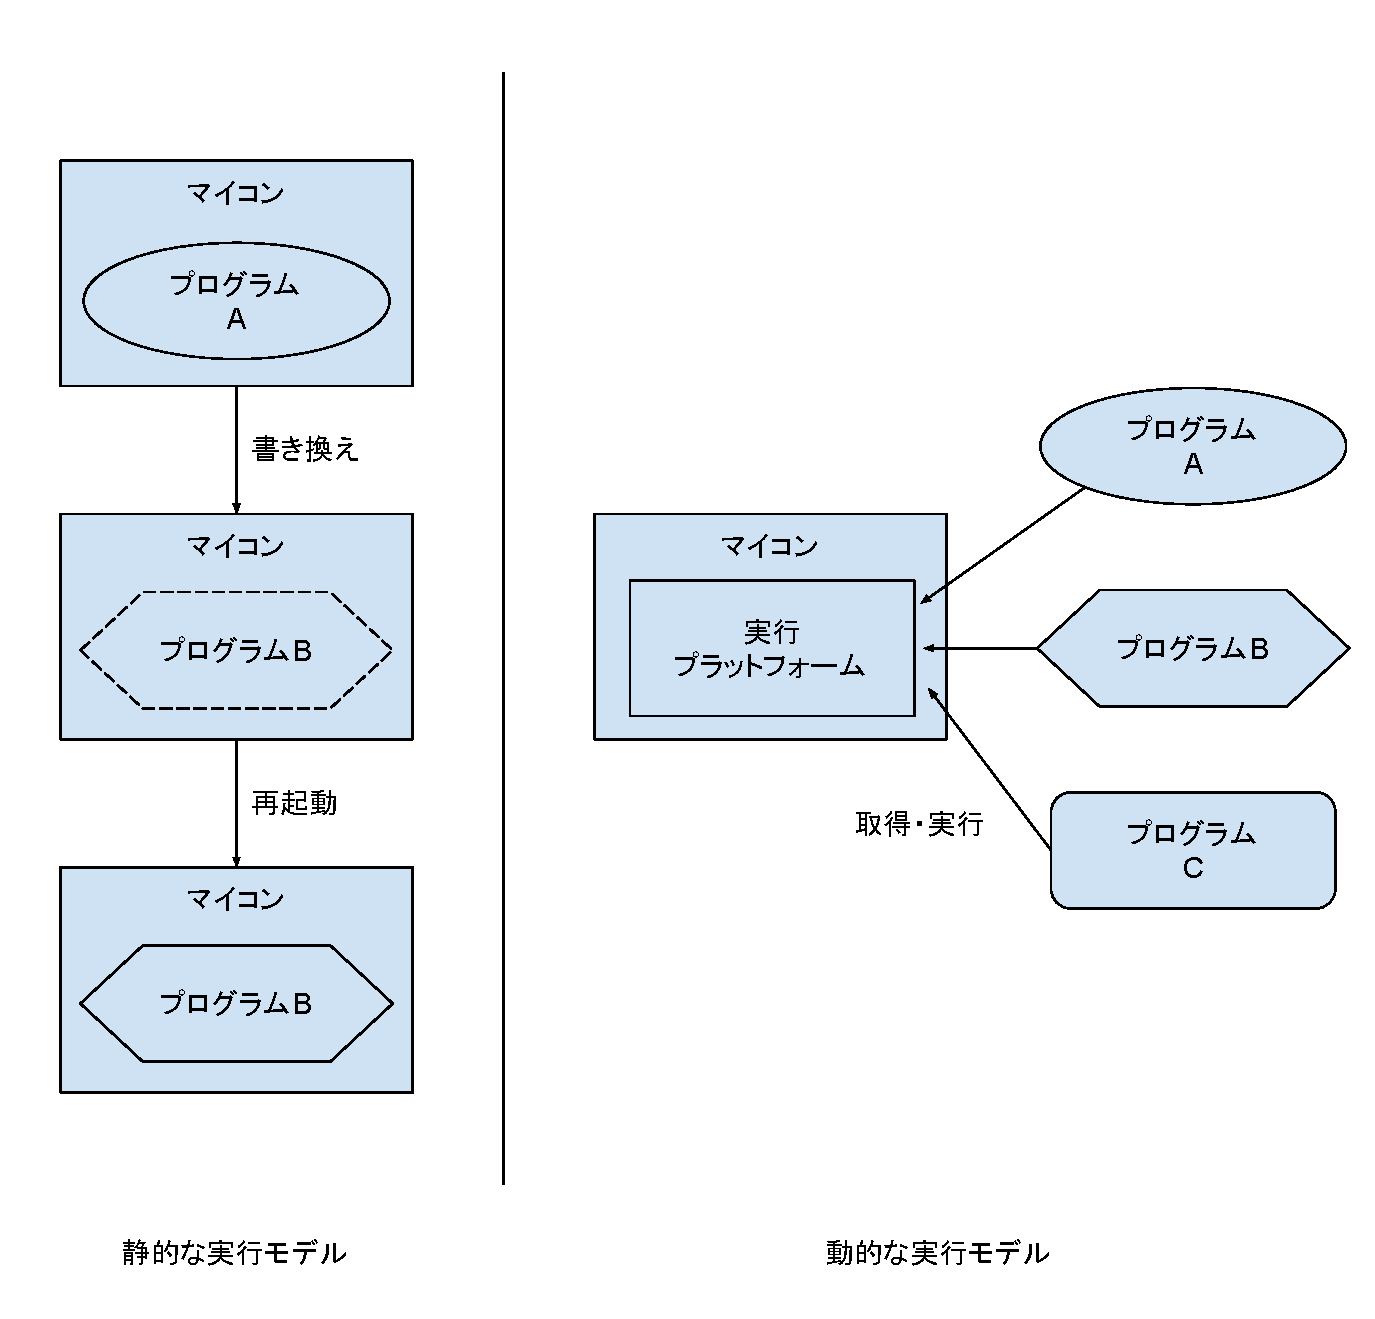
\includegraphics[bb=0 0 660 633,width=14cm]{img/static_dynamic.pdf}
  \end{center}
\end{figure}

\section{本研究の目的とアプローチ}

本研究では、WebAssemblyを実行形式として用いる事で、マイコンのような計算資源が限られた環境下でもプログラムの動的な実行ができることを示し、前述の課題を解決する。

そのために、本研究ではマイコン上でWebAssemblyバイナリの取得、実行および更新を行うための実行環境を設計した上で、その実現可能性を示すため、C言語によりWebAssemblyバイナリのインタプリタを実装し、ESP32マイコンとPC上でそれぞれ同一のWebAssemblyを実行できることを示した。
また、それぞれの環境での実行性能を、PC上のWebブラウザにおけるWebAssemblyバイナリの実行性能と比較する事で、マイコンにおけるWebAssembly実行環境の性能を検討した。

\section{本論文の構成}

本論文における以降の構成は次の通りである。

\ref{chap:related_works}章では、マイコンにおけるプログラムの更新を行うための関連技術として、MicroPythonおよびESP-IDFが提供するOTA機能について述べる。

\ref{chap:design}章では、マイコン上でWebAssemblyプログラムを取得、実行、更新するための実行環境の設計を提案する。提案する実行環境では、プログラムをHTTP通信を用いてインターネット上から取得する。プログラムは実行毎に再取得することで更新しつつ、キャッシュの活用により通信による計算負荷と帯域を削減する。

\ref{chap:implementation}章では、本研究で実装したWebAssembly実行環境について述べる。
本研究では、WebAssemblyバイナリの実行部分を実装した。ホストプログラムから静的なバイナリをパースおよびインスタンス化し、対応する関数を呼び出すことで実行する。

\ref{chap:evaluation}章では、本研究で実装したWebAssembly実行環境を用いて、ESP32マイコン上およびmacOSを搭載したPC上で同一のWebAssemblyバイナリを実行した結果と、PC上のWebブラウザで同じWebAssemblyバイナリを実行した結果を比較し、マイコンにおけるWebAssembly実行環境の性能を検討する。

\ref{chap:conclusion}章では、本研究における結論を示す。
